\documentclass[twocolumn,superscriptaddress,aps,prb,floatfix]{revtex4-1}

\usepackage{graphicx}% Include figure files
\usepackage{dcolumn}% Align table columns on decimal point
\usepackage{bm}% bold math
\usepackage{color}
\usepackage[caption=false]{subfig} 

\usepackage{listings}

\definecolor{dkgreen}{rgb}{0,0.6,0}
\definecolor{gray}{rgb}{0.5,0.5,0.5}
\definecolor{mauve}{rgb}{0.58,0,0.82}

\lstset{frame=tb,
  language=python,
  aboveskip=3mm,
  belowskip=3mm,
  showstringspaces=false,
  columns=flexible,
  basicstyle={\small\ttfamily},
  numbers=none,
  numberstyle=\tiny\color{gray},
  keywordstyle=\color{blue},
  commentstyle=\color{dkgreen},
  stringstyle=\color{mauve},
  breaklines=true,
  breakatwhitespace=true,
  tabsize=3
}

\usepackage{amsthm}
\usepackage{amsmath}
\usepackage{amssymb}


\newcommand{\figref}[1]{Fig. \ref{#1}}


\newtheorem{theorem}{Theorem}[section]
\newtheorem{lemma}[theorem]{Lemma}
\newtheorem{proposition}[theorem]{Proposition}
\newtheorem{corollary}[theorem]{Corollary}

%\newenvironment{proof}[1][Proof]{\begin{trivlist}
%\item[\hskip \labelsep {\bfseries #1}]}{\end{trivlist}}
%\newenvironment{definition}[1][Definition]{\begin{trivlist}
%\item[\hskip \labelsep {\bfseries #1}]}{\end{trivlist}}
%\newenvironment{example}[1][Example]{\begin{trivlist}
%\item[\hskip \labelsep {\bfseries #1}]}{\end{trivlist}}
%\newenvironment{remark}[1][Remark]{\begin{trivlist}
%\item[\hskip \labelsep {\bfseries #1}]}{\end{trivlist}}

%\newcommand{\qed}{\nobreak \ifvmode \relax \else
%      \ifdim\lastskip<1.5em \hskip-\lastskip
%      \hskip1.5em plus0em minus0.5em \fi \nobreak
%      \vrule height0.75em width0.5em depth0.25em\fi}

\begin{document}

%\allowdisplaybreaks

\title{How nonconvex is it? Exploring neural network geometry through Dynamic String Sampling}


\author{C. Daniel Freeman}
\email{daniel.freeman@berkeley.edu}
\affiliation{Department of Physics, University of California, Berkeley, CA 94720, USA}

\author{Joan Bruna}
\affiliation{Department of Statistics, University of California, Berkeley, CA 94720, USA}


\date{\today}

\begin{abstract}
 The natural tool for understanding neural network training is \emph{nonconvex optimization}.  In practice, this means that, for some given learning task, a loss function is optimized via some flavor of gradient descent.  While this strategy has led to great success, it is surprising that not much is known about the geometry of the loss function itself.  In this manuscript, we examine the geometry of these loss functions for several learning tasks (QUAD, MNIST).  In so doing, we provide both a quantitative handle on problem nonconvexity as well as an algorithm for estimating that nonconvexity (Dynamic String Sampling).  Operationally, given two models which have nearly the same loss $L_0$ on test data, our algorithm searches for continuous paths in the space of model parameters which do not exceed $L_0$.  Whether such a path can be found defines a notion of connectedness, and thus nonconvexity.
\end{abstract}

\maketitle


%%%%%%%%%%%%%%%%%%%%%%
%%%%%%%%%%%%%%%%%%%%%%
\section{Introduction}
\label{sec:Intro}
%%%%%%%%%%%%%%%%%%%%%%
  



	
%%%%%%%%%%%%%%%%%%%%%%
\section{Quantifying Nonconvexity}
\label{sec:QuanNoncon}

\subsection{Definitions}
\label{sec:Defs}
%%%%%%%%%%%%%%%%%%%%%%

 For a model with network parameters $\theta_i$, and a learning problem with sample space $X$, the fundamental object of study is the loss function, $L(X, \theta_i)$.  In practice, one only has access to an estimate of the loss function over some restricted subset, $\chi_i$, of the sample space: $E( L(X, \theta_i), \chi_i )$.  Unless otherwise stated, the loss functions computed throughout are assumed to be on a restricted test set not used during training.
 
 A key ingredient of the algorithm is the use of an \emph{interpolated model}.  For two given models, $\theta_1$ and $\theta_2$, we defined the interpolated model with parameter $t$ as follows:
 
\begin{equation}
\Theta (\theta_1 ,\theta_2, t) := \theta_1 (1-t) + \theta_2 t
\end{equation}

 Thus, the interpolated model parameters---i.e., weights and biases---are simply linearly interpolated between two given models.
 
 Additionally, the algorithm requires an estimate of the interpolated loss curve:

 \begin{equation}
 \gamma(\theta_1, \theta_2) := L (X ,\Theta (\theta_1, \theta_2, t)), t \in [0,1]
 \end{equation}

 or, an estimate of the loss on those models which are linear interpolations sitting between $\theta_1$ and $\theta_2$.  More specifically, we seek efficient estimates of the location of the maxima, $t^* := \frac{d \gamma(\theta_1, \theta_2, t)}{dt} \bigg|_{t^*} = 0, \frac{d^2 \gamma(\theta_1, \theta_2, t)}{dt^2} \bigg|_{t^*} < 0$.  While in principle, the interpolated loss curve could have rich structure, in practice it is generally fairly smooth, thus straightforward hill climbing algorithms can efficiently locate these points.
 
 Finally, for a pair of models $(\theta_1, \theta_2)$, it will be convenient to define the maximum interpolated error:
 
  \begin{equation}
  \Gamma(\theta_1, \theta_2) := \rm{min}_{\Theta^*(\theta_1, \theta_2)}\:\rm{max}\:L (X, \theta_i) \bigg|_{\theta_i \in \Theta^*} \label{eq:minmaxerror}
  \end{equation}
 
 where $\Theta^* (\theta_1, \theta_2)$ is \emph{any} continuous path in the space of weights connecting $\theta_1$ and $\theta_2$.  Thus, $\Gamma(\theta_1, \theta_2)$ represents the minimum possible maximum loss achieved by those paths in the space of weights connecting $\theta_1$ and $\theta_2$.  More intuitively, if $\Gamma (\theta_1, \theta_2) \leq \rm{max}\: (L(X,\theta_1), L(X,\theta_2))$, then the models are ``connected''---there exists a continuous path in the space of models with total loss never exceeding the maximum loss achieved by $\theta_1$ or $\theta_2$. 
 
 \subsection{The Greedy Algorithm}
 \label{sec:GreedyAlg}
 
 1. Train two models $\theta_i$ and $\theta_j$ to a threshold loss value, $L_0$.
 
 2. Determine the location of the global maxima, $t^*$, on the interpolated loss curve $\gamma(\theta_i, \theta_j)$. 
 
 3. Perform gradient descent on the interpolated model $\Theta (\theta_i, \theta_j, t^*) := \theta_{i,j}$ until it is below $\alpha L_0$ for some $\alpha \in [0,1]$ .
 
 4. Calculate the maxima of the interpolated losses $\gamma(\theta_i, \theta_{i,j})$ and $\gamma(\theta_{i,j}, \theta_j)$.  If these maxima are below $L_0$, then stop recursing on this branch and proceed to remaining branches(see 5).  If not, proceed to step 5.
 
 5. For those pairs, $\theta_a, \theta_b$ from step 4 for which the maxima exceeds $L_0$, start a new branch by returning to step 2 and making the replacement $i->a$ and $j->b$.  If depth exceeds $d$, stop (see below).
 
 \begin{figure}
\begin{center}
\scalebox{1}{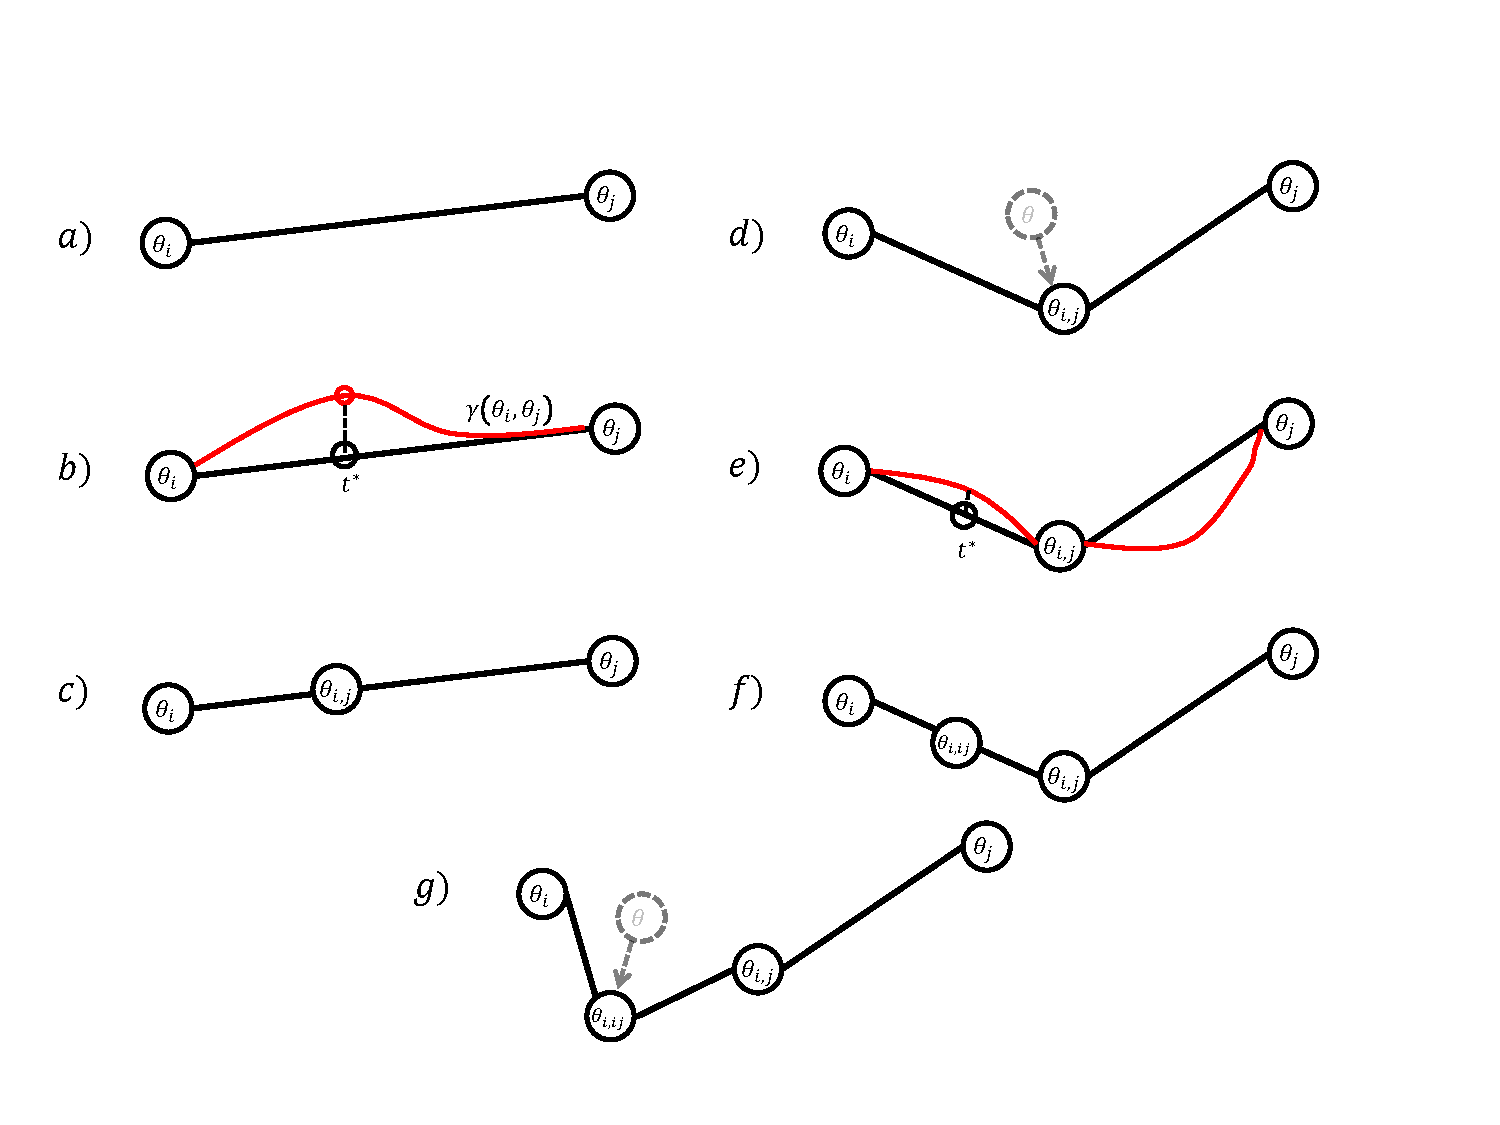
\includegraphics[width=1.0\columnwidth]{AlgorithmFigure}}
\end{center}
\caption{A cartoon of the algorithm.  $a):$ The initial two models with approximately the same loss, $L_0$. $b):$ The interpolated loss curve, in red, and its global maximum, occuring at $t=t^*$. $c):$ The interpolated model $\Theta(\theta_i, \theta_j, t^*)$ is added and labeled $\theta_{i,j}$.  $d):$ Stochastic gradient descent is performed on the interpolated model until its loss is below $\alpha L_0$. $e):$ New interpolated loss curves are calculated between the models, pairwise on a chain.  $f):$ As in step $c)$, a new model is inserted at the maxima of the interpolated loss curve between $\theta_i$ and $\theta_{i,j}$.  $g):$  As in step $d)$, gradient descent is performed until the model has low enough loss.}
\label{fig:AlgorithmFigure}
\end{figure}
 
 We provide a cartoon of the algorithm in \figref{fig:AlgorithmFigure}.  If the algorithm succeeds, then the output of the algorithm is a sequence of models, $\theta_i$ such that the pairwise interpolated loss curve between each in a sequence will be less than the threshold $L_0$.  Thus, the algorithm outputs a continuous path in parameter space connecting the original two models such that everywhere along the path, the total loss is less than or equal to the loss of the original models.
 
 As written, if a path does \emph{not} exist, then the algorithm will clearly not converge.  Thus, on top of the parameter $\alpha$, discussed below, the algorithm has an additional free parameter in the \emph{depth} chosen to explore.  For convenience, we define the string of models produced by the algorithm at depth $d$ with parameter $\alpha$ to be the \emph{interpolated string}, $S(\theta_1, \theta_2, \alpha, d)$.  These are precisely those models recursively generated by the algorithm in step 3.  Further, these models are naturally ordered along a path, starting from $\theta_1$ and terminating on $\theta_2$, as indicated in \figref{fig:AlgorithmFigure}.
 
 Finally, to use this as a tool to diagnose convexity, we define the \emph{maximum interpolated error at depth $d$ and tolerance $\alpha$}:
 
 \begin{align}
 \tilde{\Gamma}( \theta_1, \theta_2, d, \alpha ) &:= \rm{max}\ \gamma(\theta_i, \theta_j, t)\\ \notag
 &i,\ j\ \rm{neighbors\ in}\ S(\theta_1, \theta_2, \alpha, d)
 \end{align}
 
 where by ``neighbors in $S(\theta_1, \theta_2, \alpha, d)$'', we only mean that the models are immediately adjacent on the interpolating string.  This quantity upper bounds the true maximum interpolated error, i.e. \eqref{eq:minmaxerror}.
 
 In summary: the algorithm recursively produces and trains new models lying on a continuous path in the space of model parameters, i.e. a string.  Training via gradient descent biases the path towards valleys on the loss surface, thus encouraging the loss along this path to be low.  In practice, the parameter $\alpha$ is chosen to be less than 1 to aid convergence.  We provide numerical and theoretical evidence for this choice in section SECTIONGOHERE.
 

  \subsection{Constrained Dynamic String Sampling}
  \label{sec:ConstrainedAlg}
  
  While the algorithm presented in Sec. \ref{sec:GreedyAlg} is fast for sufficiently smooth families of loss surfaces with few saddle points, here we present a slightly modified version which, while slower, provides more control over the convergence of the string.  Instead of training intermediate models via full SGD to a desired accuracy, intermediate models will be subject to a constraint that ensures they are ``close'' to the neighboring models on the string.  Specifically, intermediate models will be constrained to the unique hyperplane in weightspace equidistant from its two neighbors.  This is similar to a sort of ``$L_1$ regularization'' where the loss function for a given model on the string, $\theta_i$, has an additional term $\tilde{L}(\theta) = L(\theta)+\zeta(\|\theta_{i-1} - \theta_i\|+\|\theta_{i+1} + \theta_i\|)$.  The strength of the $\zeta$ regularization term controls the ``springy-ness'' of the weightstring. note: make this more precise, the hyperplane constraint is stronger than the $L_1$ constraint...$L_1$ only keeps the model in a ball close to the midpoint between the models.
  
  Because adapting DSS to use this constraint is straightforward, here we will describe an alternative ``breadth-first'' approach wherein models are trained in parallel until convergence.  This alternative approach has the advantage that it will indicate a disconnection between two models ``sooner'' insofar as it will be clear two models cannot be connected once the loss on either of the two initial models, $\theta_1$ or $\theta_2$, is less than $\Gamma(\theta_1, \theta_2)$.  The precise geometry of the loss surface will dictate which approach to use in practice.
  
  Given two random models $\sigma_i$ and $\sigma_j$ where $|\sigma_i - \sigma_j| < \kappa$, we aim to follow the evolution of the family of models connecting $\sigma_i$ to $\sigma_j$.  Intuitively, almost every continuous path in the space of random models connecting $\sigma_i$ to $\sigma_j$ has, on average, the same (high) loss.  For simplicity, we choose to initialize the string to the linear segment interpolating between these two models.  If this entire segment is evolved via gradient descent, the segment will either evolve into a string which is entirely contained in a basin of the loss surface, or some number of points will become fixed at a higher loss.  These fixed points are difficult to detect directly, but will be indirectly detected by the persistence of a large interpolated loss between two adjacent models on the string.
  
  The algorithm proceeds as follows:
  
  (0.) Initialize model string to have two models, $\sigma_i$ and $\sigma_j$.
  
  1. Begin training all models to the desired loss, keeping the instantaneous loss of all models being trained approximately constant..
  
  2. If the pairwise interpolated loss $\gamma(\sigma_n,\sigma_{n+1})$ exceeds a tolerance $\alpha_1$, insert a new model at the maximum of the interpolated loss between these two models.  For simplicity, this tolerance is chosen to be $(1 + \alpha_1^*)$ times the instantaneous loss of all other models on the string.  
  
  3. Repeat steps (1) and (2) until all models (and interpolated errors) are below a threshold loss $L_0$, or until a chosen failure condition (see \ref{sec:Fail}).
  
  \subsection{Failure Conditions}
  \label{sec:Fail}
  
  While the algorithms presented will faithfully certify two models are connected if the algorithm converges, it is worth reemphasizing that they do not guarantee that two models are disconnected if the algorithm fails to converge.  In general, the problem of determining if two models are connected can be made arbitrarily difficult by choice of a particularly pathological geometry for the loss function, so we are constrained to heuristic arguments for determining when to stop running the algorithm.
  
  Thankfully, in practice, loss function geometries for problems of interest are not intractably difficult to explore.
 

 %%%%%%%%%%%%%%%%%%%%%%
\section{Analytic Toy Model}
\label{sec:ToyModel}

\subsection{The Linear Case}
\label{sec:LinToy}

 To build intuition for the nonlinear case, here we treat an ``almost linear'' regression task.  The strategy will be first, to understand how dynamic string sampling applies in an analytically tractable model, and second, to leverage this intuition for the more complicated numerical systems to follow.  We will proceed by studying the level sets of the \rm{QUARTICLOSS} toy model defined as followed:
 
 For weight matrices $w_1, w_2$, input column vectors $x_i$ of dimension $d_1$, and output scalars $y_i$, suppose we aim to minimize the loss function
 
  \begin{equation}
 L(w_1,w_2)=(w_1 w_2 x - y)^2 \label{eq:losseq}
  \end{equation}
 
 For simplicity, suppose $w_1$ is a row vector with dimension $d_2$.  This fixes the dimension of $w_2$ to $d_1$ by $d_2$.
 
 Suppose we are given the globally optimal $w_1^*$ and $w_2^*$ which minimize $L$.  These weights are not unique, because we can reparameterize the global optima in the following way:
 
  \begin{align}
 w_1^* &\rightarrow \rm{any\ nonzero\ vector} = w_1 \\
 w_2^* &\rightarrow \frac{w_1^T}{||w_1||} a^* + \alpha (w_1^T)_\perp a^*
  \end{align}
  
  where $a^*$ is the row vector $a^*=w_1^* w_2^*$ which globally optimizes \eqref{eq:losseq}, and $\alpha$ is an arbitrary scalar.  This freedom represents an internal symmetry of the weights.
  
  Given two models $w_1^A w_2^A = a^*$ and $w_1^B w_2^B = a^*$, let $w_1^A \cdot w_1^B=||w_1^A||||w_1^B||\rm{cos}\theta$.  Either can be continuously connected to the other via the following two steps.  Without loss of generality, we will connect the $A$ components to the $B$ components.  First, the component of $w_2^A$ perpendicular to $w_1$ is scaled linearly from its original value $\alpha$ to $\alpha^*$:
  
 \begin{equation}
 w_2^A = \frac{w_1^T}{||w_1||} a^* + (w_1^T)_\perp a^* \rightarrow \frac{w_1^T}{||w_1||} a^* + \alpha^* (w_1^T)_\perp =: w_2^{**}
  \end{equation}
  
 Where $\alpha^*=\frac{1-||w_1^B||\rm{cos}\theta}{||w_1^B|| \rm{sin}\theta}$.  Defined in this way, $w_2^{**}$ now satisfies both $w_1^A w_2^{**} = a^*$ as well as $w_1^B w_2^{**} = a^*$.  Then, simple linear interpolation connects $w_1^A$ to $w_1^B$:
 
  \begin{equation}
 w_1^a \rightarrow w_1^a (1-t) + w_1^b t
  \end{equation}
  
  Finally, the same procedure can connect $w_2^B$ to $w_2^A$, continuously and invertibly, thus we are done.
  
  Thus, linearly scaling first $\alpha$ to $\alpha^*$ and then scaling $t$ from $0$ to $1$ connects $w_1^A$ to $w_1^B$.  Crucially, the entire procedure preserves the global minimum of the loss function.  
  
  (Alternate proof from Yasaman Bahri): Alternatively, one can first connect $w_1^a$ to $w_1^b$ via the linear transformation $w_1^b =  w_1^a O$.  This can be done continuously via the lie algebra element $g$ defined by $O := \rm{exp}[g]$.

 \begin{align}
 w_1^a w_2^a &\rightarrow w_1^a e^{t_1 \bold{g}} e^{-t_1 \bold{g}} w_2^a \\ \notag
 &\rightarrow (w_1^a e^{t_1 \bold{g}}) ( e^{-t_1 \bold{g}} w_2^a)
  \end{align}
  
  This continuously connects $w_1^a$ to $w_1^b$.  The loss remains fixed because the term $e^{t_1 \bold{g}} e^{-t_1 \bold{g}}$ always acts as the identity.  Then, after scaling $t_1$ from $0$ to $1$, one can linearly interpolate between $\rm{exp} (-g) w_2^a$ and $w_2^b$, again leaving the loss invariant:
  
  \begin{equation}
 e^{-\bold{g}} w_2^a \rightarrow (1-t_2) e^{-\bold{g}} w_2^a + t_2 w_2^b
  \end{equation}
 
  Now that we have shown a continuous path exists for this internal symmetry, it remains to be shown that DSS will faithfully produce a continuous path.  For DSS, the relevant interpolation equations are:
  
  \begin{align}
  w_1(t) &= w_1^A (1-t) + w_1^B t \\
  w_2(t) &= w_2^A (1-t) + w_2^B t
  \end{align}
  
  Examining $w_1(t) w_2(t)$, the first and last terms in the product yield $(1-t)^2 a^* + t^2 a^*$.  The remaining cross terms can be rewritten as $\gamma t(t-1) a^*$ for a constant $\gamma$.  Because we are promised that $A$ and $B$ are global minima in the space of weights, the loss is either constant along the path, or reaches a reaches a global maxima somewhere, which we call $t^*$.  In the former case, we are done, because DSS will have provided a continuous path in the space of weights with nonincreasing loss.
 
  In the latter case, consider the hyperplane splitting $A$ and $B$.  Because the loss function is continuous, and because we have demonstrated the existence of a continuous path in weight space connecting $A$ to $B$, this path must puncture the hyperplane somewhere.  We assume, but do not prove here, that constrained gradient descent on the hyperplane will find this new global minima.  We comment on this assumption more below.  Call this point $\pi_1$, and the associated weights $w^{\pi_1}_1$ and $w^{\pi_1}_2$.
  
  Recursively splitting the weight string and performing gradient descent on the resulting constraining hyperplanes provides a sequence of points (reordered sequentially from $A$ to $B$) ${\pi_1, \pi_2, ..., \pi_n}$ where $n = \Sigma_{i=0}^{d} 2^i$ for depth $d$ recursive splits.  By the smoothness of the loss function, the maximum interpolated error along the path $A, \pi_1, ..., \pi_n, B$ can be bounded above to $L_0 + \epsilon$ for any $\epsilon > 0$ so long as $d$ is made sufficiently large, where $L_0$ is the globally minimum loss achieved by $a^*$.
  
  This bound can be made more precise...
  
  ...Need to complete this argument still...
  we note that $\nabla L \bigg|_{t^*}...$
  
  
  
\subsection{The Nonlinear Case}
\label{sec:NonlinToy}

The most immediate, theoretically tractable nonlinear analogue of the model studied in \ref{sec:LinToy} is the same model with a Relu nonlinearity as studied by (cite people):

  \begin{equation}
 L(w_1,w_2)=(w_1 \rm{max} (w_2 x, 0) - y)^2 \label{eq:losseq}
  \end{equation}
  
  ... ...
  
 
 %%%%%%%%%%%%%%%%%%%%%%
\section{Symmetries}
\label{sec:Symm}

When trying to understand the geometry of a loss function, it's imporant to distinguish between symmetries intrinsic to an architecture versus symmmetries within the loss function itself.  In practice, essentially all neural networks currently used possess the discrete symmetry defined by permutation of neurons.  RELUs without bias also have a well known continuous scaling symmetry[cite].  [cite https://arxiv.org/pdf/1511.01029.pdf].

Intuitively, one might hope to promote the immense discrete symmetry groups possessed by a given architecture to a larger continuous subgroup of $SO(N)$.  This clearly does not hold in absolute generality, but one could imagine looking at the neighborhood of a permutation on the full group, $SO(N)$, and piecewise gluing together these neighborhoods (see Yasaman's argument again).  In general, this will depend on both the density of available permutations, as well as the maximum curvature of the loss with respect to variations in the weights about these fixed permutations (i.e., $\frac{\partial^2 L}{\partial w_i \partial w_j}$).  If this maximum, call it $\kappa$ does not scale too poorly with increasing model size (i.e., more neurons per layer and more layers), then the expectation is that \emph{any} model at a fixed loss $L_0$ can be continuously connected to any other model at fixed loss $L_0$ while keeping the loss fixed (or at least nonincreasing).  

This expectation is intuitively consistent with the notion that a model with many more parameters than samples in training/test sets will have more ``wiggle room'', by sheer size of the dimensionality mismatch---a model in the ``continuum limit'' will have so many more dimensions that varying weights at a fixed loss should be easy.  This ``wiggle room'' appears because most directions simply have no effect on the value of the loss at all.

Of course, a loss function can be adversarially generated which explicitly possesses disconnected components, but this sort of disconnection is pathological.  Thus, we aim to explore the following question: Are there any problems of practical interest where two ``equivalent'' model solutions cannot be continuously connected to one another?


 
 
 %%%%%%%%%%%%%%%%%%%%%%
\section{Numerical Experiments}
\label{sec:NumExp}

For our numerical experiments, we aimed to extract qualitative features of both small, toy networks, as well as of larger workhorse networks suitable for use on real world tasks (e.g. MNIST).  At its core, the maximum interpolated error (i.e., \eqref{eq:minmaxerror}) is a measure of problem nonconvexity---or, more precisely, of the nonconvexity of the loss surface of a given architecture on a particular learning problem.

Most remarkably, we always found that models trained to the same loss on the training set were part of the same connected component.  In other words, DSS was always able to efficiently generate a continuous path in the space of models with loss lower than or equal to the the loss of the models on the endpoints.  This was true even for models ``far apart'' in weight space.  This may be a quirk of the problems studied, but might point towards a more general consequence of the tremendous internal symmetries intrinsic to common neural network architectures.  We comment more on this in the discussion.

Because connecting models was in some sense ``easy'', we collected statistics for the resulting strings in model space.  Particularly natural quantities of interest are the length of the model strings---normalized by the end-to-end displacement of the string---as well as the average angle subtended by discrete segments of the model string.  Intuitively, these measures provide information about the curvature of the level sets, and hence provide indirect information about the nonconvexity of the loss surface.

For the convnet implementation of MNIST, we qualitatively examined how the receptive fields of the first feature layer transformed along the continuous paths provided by DSS.


\subsection{Polynomial Regression}
\label{sec:PolyFuncs}
%%%%%%%%%%%%%%%%%%%%%%

 Polynomial function regression is a task for which small neural networks can achieve extremely high accuracy.  For our numerical experiments, we studied a 1-4-4-1 fully connected multilayer perceptron style architecture with RELU activation and RMSProp optimization.  For ease-of-analysis, we restricted the family of polynomials to be strictly contained in the interval $x\in[0,1]$ and $f(x)\in[0,1]$.
 
 Discussion of different Loss functions
 
 etc.


%%%%%%%%%%%%%%%%%%%%%%
\subsection{MNIST}
\label{sec:MNIST}
%%%%%%%%%%%%%%%%%%%%%%


%%%%%%%%%%%%%%%%%%%%%%
%%%%%%%%%%%%%%%%%%%%%%
\section{Discussion}
\label{sec:Discussion}
%%%%%%%%%%%%%%%%%%%%%%

 
 

\bibliography{nonconvex}

\end{document}
%
% {**}{**}{**} End of file apssamp.tex {**}{**}{**}
